\documentclass{article}


%............Inicia Preambulo.......................
\usepackage{graphicx}
\usepackage{float}
\usepackage[utf8]{inputenc}
\usepackage[shortlabels]{enumitem}
\usepackage{textcomp}
\usepackage{multicol}
\usepackage{caption}
\usepackage[spanish]{babel}
\usepackage[total={17.5cm, 23cm}, top=2cm, left=2cm]{geometry}
\usepackage{esvect}
\usepackage[font=footnotesize]{caption}

\spanishdecimal{.}
\parindent 0cm

%.............Fin de Preambulo........................


\begin{document}

\begin{center}
{\Large \textbf{Universidad Autónoma de Coahuila}}
\end{center}

\begin{center}
{\large Facultad de Ciencias Físico-Matemáticas}
\end{center}

%Materia
\begin{center}
{\large Metodos Numericos}
\end{center}

%Título
\begin{center}
{\large Conversiones bases y errores de computadora}
\end{center}

%Fecha
\begin{center}
{\large 28 de Noviembre del 2019}
\end{center}

%Autor
\begin{center}
{\large José Antonio Olveda García}
\end{center}

\vspace{5mm}

\begin{multicols}{2}

%\section{Objetivo}
%\label{sec:obj}
  

\section{Introducción}
\label{sec:intro}
Una de las implicaciones de trabajar con aritmetica computacional es que los numeros tiene una representacion finita, es decir, los numeros se almacenan con un numero infinito de digitos.
A continuacion se describe el sistema de aritmetica de un punto flotante de las computadoras, tambien conocida como \textbf{Conjunto de numeros en la maquina de numero flotante} 

\section{Sistema Numerico}
\label{sec:Sis}
\textbf{Sistema Numerico}
\textbf{Numeracion de base diez (sistema decimal)}
El sistema que se utiliza de manera habitual para representar los numeros y trabajar con ellos es el sistema posicional de base 10. El cual se divide en 10 caracteres diferentes llamadas digitos y la magnitud depende de la posicion del digito.
Ejemplo de numeros en base 10 \\
\begin{center}
$261$ \\
$2458.45$\\
\end{center}
Estos numeros tambien tienen su representacion en el sistema posicional de base 10 de la siguiente manera
\begin{center}
$261=2x10^{2}+6x10^{1}+1x10^0$
\\
$2458.456=2x10^{3}+4x10^{2}+5x10^1+8x10^{0}+4x10^{-1}+5x10^{-2}+6x10^{-3}$
\\
\end{center}
Lo que significa que cualquier numero entero Z se representa como un polinomio en base 10 con coeficientes enteros $a_{i}$ entre 0 y 9.
Aun cuando las computadoras usan sistema binario los usuarios prefieren trabajar en el sistema decimal que es mas familiar cuando se quieren dar datos a la computadora y del sistema binario al decimal, cuando se obtiene datos en la computadora
\section{Conversion de numeros enteros del sistema decimal a un sistema base b y viceversa}
\label{sec:Conversion de numeros enteros del sistema decimal a un sistema base b y viceversa}
Para Para convertir un numero n del sistema  decimal a un sistema base b (en este caso base 2) son considerados el cociente y el residuo resultantes; se divide $c_{1}$ en la base b y se anota el nuevo cociente $c_{2}$ y el nuevo residuo. Este procedimiento se repite hasta obtener un cociente $c_{i}$ igual a cero y un residuo $r_{i}$, donde $0<r_{i}<b$. El equivalente a n en el sistema de base b queda formado asi
\\
\begin{equation}
(r_{i-1},r_{i-2},...,r_{i})
\end{equation}
De (1) tenemos que el $358_{10} = 101100110_{2}$
\\
Para convertir un entero m de un sistema base b al sistema decimal se multiplica cada digito de m por la base b elevada a una potencia igual a la posicion del digito, tomando como posicion cero la del digito mas a la derecha.\\
La suma da el equivalente al decimal\\
Ejemplo
\begin{center}
$101100110_{2}=1x2^{8}+0x2^{7}+1x2^{6}+1x2^{5}
+0x2^{4}+0x2^{3}+1x2^{2}+1x2^{1}+0x2^{0}$   
\end{center}

\section{Conversion de numeros fraccionarios del sistema decimal a un sistema de base b}
\label{sec:conver}
Se multiplica por la base b; al resultado que tiene una parte entera y una parte fraccionaria $f_{1}$. Si multiplica ahora $f_{1}$ por b y se alterna un nuevo producto con parte entera $a_{2}$ y fraccionaria $f_{1}$.
\\
Este procedimiento se repite un numero suficiente de veces hasta que se presenta $0f_{n}=0$. El equivalente en $x_{10}$ en base b y queda asi 
\begin{center}
$0.e_{1}e_{2}e_{3}$
\end{center}
Ejemplo 
\\
Convertir el numero $0.2_{10}$ a binario
\\
\\
\begin{tabular}{|r|r|r|r|}
\hline
 & Frac decxbase &par ent. y frac & res$-$par ent\\
\hline
1 & 0.2x2 & 0.4 & 0.4-0=0.4 \\
\hline
2 & 0.4x2 & 0.8 & 0.8-0=0.8 \\
\hline
3 & 0.8x2 & 1.6 & 1.6-1=0.6 \\
\hline
4 & 0.6x2 & 1.2 & 1.2-1=0.2 \\
\hline
5 & 0.2x2 & 0.4 & 0.4-0=0.4 \\
\hline
\end{tabular}
Despues de $r_{4}$ se repite indefinidamente, por lo que $0.2_{10}=0.001100110011..._{2}$. A este tipo de fraccion se le llama fraccion que no termina, y hay otras que son llamadas fracciones que terminan
\\
Ejemplo
\begin{center}
$1/4=0.25_{10}$
\end{center}
\begin{tabular}{|r|r|r|r|}
\hline
 & Frac decxbase & par ent. y frac. & res-par ent \\
 \hline
1 & 0.25x2 & 0.5 & 0.5-0=0\\
 \hline
2 & 0.5x2 & 1.0 & 1.0-1=0\\
 \hline
\end{tabular}
\\
\\
entonces $0.25_{10}=01_{2}$
\\
De lo anterior puede observarse que 
\\
\begin{center}
$358.2_{10}=101100110.0011001100110011..._{2}$
\end{center}
Se puede afirmar que cualquier numero entero a fraccionario se pueden trabajar por separado y despues se pueden integrar
\section{Conversion de numero fraccionario en sistema binario a sistema decimal}
\label{sec:Con}
El procedimiento es similar a el de numeros enteros, solo hay que tomar la posicion inicial con -1, apartir del punto 
\\
Ejemplo
\\
Convierta $0.010101110_{2}$ a decimal 
\\

$0.010101110=0x2^{-1}+1x2^{-2}+0x2^{-3}+1x2^{-4}+0x2^{-5}+1x2^{-6}+1x2^{-7}+1x2^{-8}+0x2^{-9}=0.33984375_{10}$
\\
\textbf{Manejo de numeros en la computadora}
\\
Por razones practicas, solo puede manejarse una cantidad finita de bits para cada numero en la computadora y esta cantidad o longitud varia de una maquina a otra. Por ejemplo, cuando se realizan calculos de ingenieria y ciencias es deseable una longitud grande; por otro lado una longitud pequeña es mas economica y util en la computadora empleada en calculos y procesos administrativos. Para una computadora dado el numero de bits generalmente se llama palabra. Las palabras van desde 8 bits hasta 64 bits.
\\
Para facilitar su manejo, la palabra se divide en partes mas cortos denominadas bytes; por ejemplo, una palabra de 32 bits puede dividirse en 4 bytes (8 bits cada uno)
\section{Tipos de errores}
\label{sec:Tipos}
Los tipos de errores de medicion pueden ser aleatorios, sistematicos, despreciativos o significativos, etc.
\\
Se le conoce como error de medicion a la diferencia existente entre el valor que se ha obtenido y el valor medido 
\begin{equation}
E_{A}=|V_{R}-V_{0}|
\end{equation}
\\
Ademas de los errores despreciables y significativos, existen otros tipos de errores de medicion. Algunos se deben a defectos de los instrumentos empleados y otros al mal manejo de los instrumentos por parte de la persona que lleva a cabo la medicion.
\\
\\
\textbf{ERROR ALEATORIO}
\\
son aquellos que se dan cuando se hacen medidas consecutivas de un mismo objeto o fenómeno, obteniendo valores diferentes en cada caso.
\\
En las ciencias sociales los errores aleatorios están representados por condiciones que afecten de manera particular a un miembro de la muestra que está siendo analizada.
\\
Ejemplo
\\
Se está estudiando el desempeño de un grupo de alumnos en los deportes. Hay cientos de elementos que afectan a cada joven, como las horas de sueño que ha tenido, el humor, la condición física, entre otros.
Cabe destacar que estas condiciones no intervienen en la actuación del grupo, sino en la de un solo individuo, lo que añade diferencias interesantes en los datos obtenidos.
\\
\\
\textbf{ERROR SISTEMATICO}
\\
A diferencia de los errores aleatorios, los errores sistemáticos dependen directamente del sistema que se está empleando para realizar la medición. Por este motivo, son errores constantes.
\\
Si se emplean instrumentos descalibrados, estos arrojarán medidas erróneas. El error se va a presentar incluso si se repite el proceso de medición.
En las ciencias sociales, el error sistemático se produce cuando hay una condición que afecte de manera general el desempeño de todos los individuos de la muestra.
\\
Ejemplo
\\
Un grupo de estudiantes debe presentar un examen sorpresa sobre un contenido que no se ha visto a profundidad en clases.
Se espera que el resultado de la evaluación sea pobre en cada caso, lo que representa un error sistemático.
\\
\\
\textbf{ERROR DESPRECIATIVO}
\\
Es aquel error que, por ser mínimo, no constituye un problema para las mediciones que se están llevando a cabo.
\\
Ejemplo
\\
Si se está trabajando en metros y la medida varía por 1 milímetro, se considera que este error no es significativo y el resultado se acepta como correcto.
\\
\\
\textbf{ERROR SIGNIFICATIVO}
\\
El error significativo es aquel que representa un problema para el trabajo que se está realizando. Si la diferencia de medidas es muy grande, evidentemente se tratará de un error significativo.

Hay casos en los que la diferencia es mínima pero igualmente es significativa.
\\
Ejemplo
\\
Cuando se preparan soluciones valoradas (aquellas que requieren medidas precisas de soluto y solvente), un error en la medición de los componentes siempre será significativo.
\\
\\
\textbf{ERROR POR DEFECTOS EN EL INSTRUMENTO EMPLEADO}
\\
Muchos de los errores que se cometen al momento de hacer mediciones pueden ser atribuidos a los instrumentos que se emplean.
\\
Existen algunos instrumentos que requieren ser calibrados para que las medidas obtenidas sean precisas.
\\
Los termómetros deben ser sometidos a mantenimiento y calibración cada cierto tiempo, para que no existan errores significativos en las medidas de la temperatura.

Ejemplo
\\
Los defectos de fábrica, las deformaciones y otras imperfecciones son algunos ejemplos de los causantes de errores. Asimismo, los instrumentos están sujetos a desgastarse por el uso.
\\
\\
\textbf{ERROR CAUSADO POR LA PERSONA QUE TOMA LA MEDIDA}
\\
El ser humano es imperfecto. Por lo tanto, cuando un individuo es el encargado de tomar las mediciones, existe un margen de probabilidades de que se cometa un error.

Ejemplo
\\
Si se está midiendo el volumen de un líquido en un cilindro graduado, es necesario que el operador sitúe los ojos al nivel del instrumento para obtener una medida precisa.

Si el observador sitúa la vista más arriba o más abajo de la marca, se producirá un error de medición. Este tipo de error es conocido como error de paralelaje y es uno de los más comunes.

Si el observador tiene problemas de visión o es muy descuidado, puede cometer errores al anotar los datos. Por ejemplo, un 3 puede ser confundido con un 8, lo que genera un error significativo.
\\
\\
\textbf{ERROR DEBIDO A LAS CONDICIONES AMBIENTALES}
\\
Las temperaturas, el sonido y otros estímulos del ambiente también afectan las mediciones.

Ejemplo
\\
Muchos materiales son propensos a variar en su longitud de acuerdo con el aumento y la disminución de la temperatura.

Si se están haciendo mediciones con base en la intensidad del sonido, el ruido excesivo puede dar lugar a errores.

En las balanzas, el polvo acumulado puede generar diferencias en las mediciones. En la mayoría de los casos, se tratará de errores despreciables.
\section{Como convertir de sistema decimal a Octal y viceversa}
\label{sec:Como}
Veamos el método para pasar del sistema decimal al sistema octal mediante un ejemplo. Escribiremos el número 
$768_{10}$ (base 10) en base 8:

Dividimos el número entre 8:
\begin{figure}[H]	
\centering
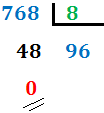
\includegraphics[scale=1]{Octal-1.png}
\caption{Situacion inicial del cambio de base}
	\end{figure}

Si el cociente es mayor o igual que 8, lo dividimos entre 8.
\\
En nuestro caso, el cociente es 96 (mayor que 8), por lo que lo dividimos de nuevo:

\begin{figure}[H]	
\centering
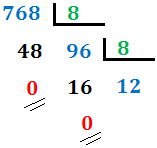
\includegraphics[scale=1]{Octal-2.png}
\caption{Division entre 8}
	\end{figure}

Continuamos así hasta obtener un cociente menor que 8.
\\
En nuestro caso, el cociente es 12 (mayor que 8), así que lo dividimos de nuevo:
\begin{figure}[H]	
\centering
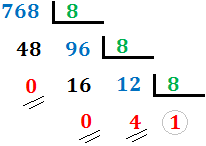
\includegraphics[scale=1]{Octal-3.png}
\caption{Procedimiento final}
	\end{figure}
El cociente es 1, menor que 8, con lo que hemos terminado el proceso. Hemos indicado los restos con dos rayas y el último cociente con una circunferencia.
\\
\textbf{El número en base 8 es:
\\
(Último cociente) (Último resto) (Penúltimo resto)... (Segundo resto) (Primer resto).}

En nuestro caso,

El último cociente es 1.

El último resto es 4.

El penúltimo resto es 0.

El primer resto es 0.

Por tanto, el número 768 en base octal es 1400. Es decir,
\begin{center}
$1400_{8}=768_{10}$
\end{center}
\textbf{¿Como convertir de base 8 a base 10?}
\\
El método que seguiremos para pasar un número en base octal a base decimal es:
\\
De derecha a izquierda: multiplicamos la primera cifra por 1 (1 es 80) ; la segunda, por 8 (8 es 81); la tercera, por 82; la cuarta, por 83. Y así hasta que hayamos multiplicado todas las cifras.
\\
Sumamos cada uno de los valores obtenidos.

Ejemplo: pasamos el número $156_{8}$ a base 10:
\begin{center}
$(6)(1)=(65)(8)=(401)(82)=(1)(64)=64$
\end{center}
El número $156_{8}$ en base 10 es
\\
\begin{center}
$6+40+64=110$
\end{center}
Podemos escribir directamente:
\begin{center}
$156=(1)(82)+(5)(8)+(6)(80)=110$
\end{center}
\section{Como convertir del sistema octal al binario y viceversa}
\label{sec:Como}
El método para convertir u numero del sistema octal a el sistema binari es realmente fácil, una persona podría ver la primera imagen en esta entrada, entender he irse sin necesidad de leer nada, pero para los que decidieron leer, aqui hay ua explicacion u poco mas compleja:
\\
Se nos da un numero:
\\
\\
1723
\\
\\
Lo separamos en sus digitos
\\
\\
1       7       2       3
\\
\\
Les asignamos valores binarios a cada dígito - los valores estan mas arriba
\\
\\
1=001 7=111 2=010 3=011
\\
\\
Por ultimo los escribimos es ese orden
\\
\begin{center}
001111010011
\end{center}
y nuestro numero ahora es binario.
La consideracion que se tomo en este caso fue la siguiente tabla
\begin{center}
1=001
\\
2=010
\\
3=011
\\
4=100
\\
5=101
\\
6=110
\\
7=111

\end{center}
\section{Visualizacion del programa}
\label{sec:Vis}
A partir de la explicacion anterior el programa implementa dichos usos en un programa de computadora que facilite todo el procedimiento para llegar al resultado y obtengamos esto mas facil y rapido
\begin{figure}[H]	
\centering
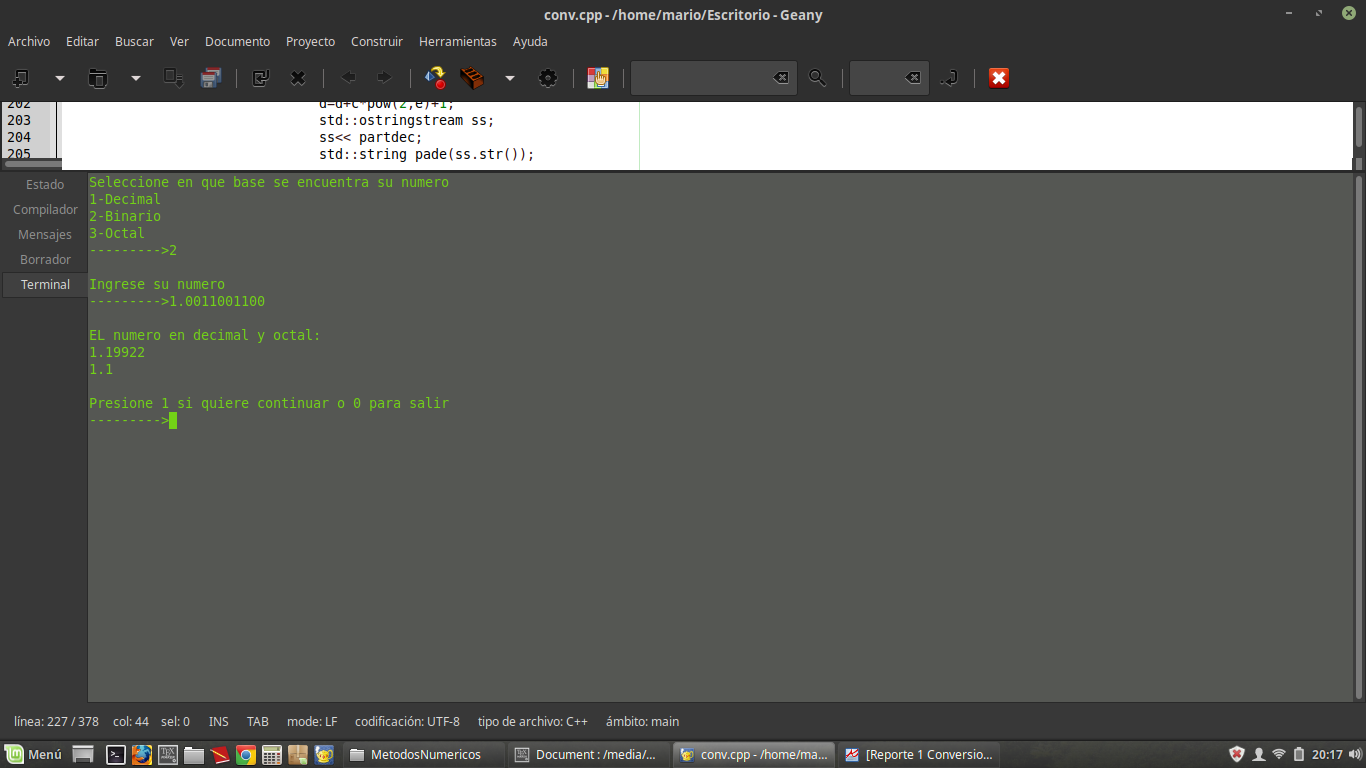
\includegraphics[scale=0.125]{Conversion.png}
\caption{Parte del programa aplicado}
	\end{figure}
Como podemos observar en la figura 4, el cambio de base de binario a decimal ahora se redujo en vez de darnos 1.2 nos dio el valor de 1.19922, esto se debe debido a que el numero de decimales tomados hace que mi valor 1.2 se haga finito, y 1.2 es un numero infinito que nunca terminara, por lo tanto es correcta la aproximacion que se establece. 
\\
Transformando de Decimal a octal se ejecuto el programa para realizar el mismo segmento que hace como con la explicacion anterior, tomaremos el mismo numero que se considero en el ejemplo
\begin{figure}[H]	
\centering
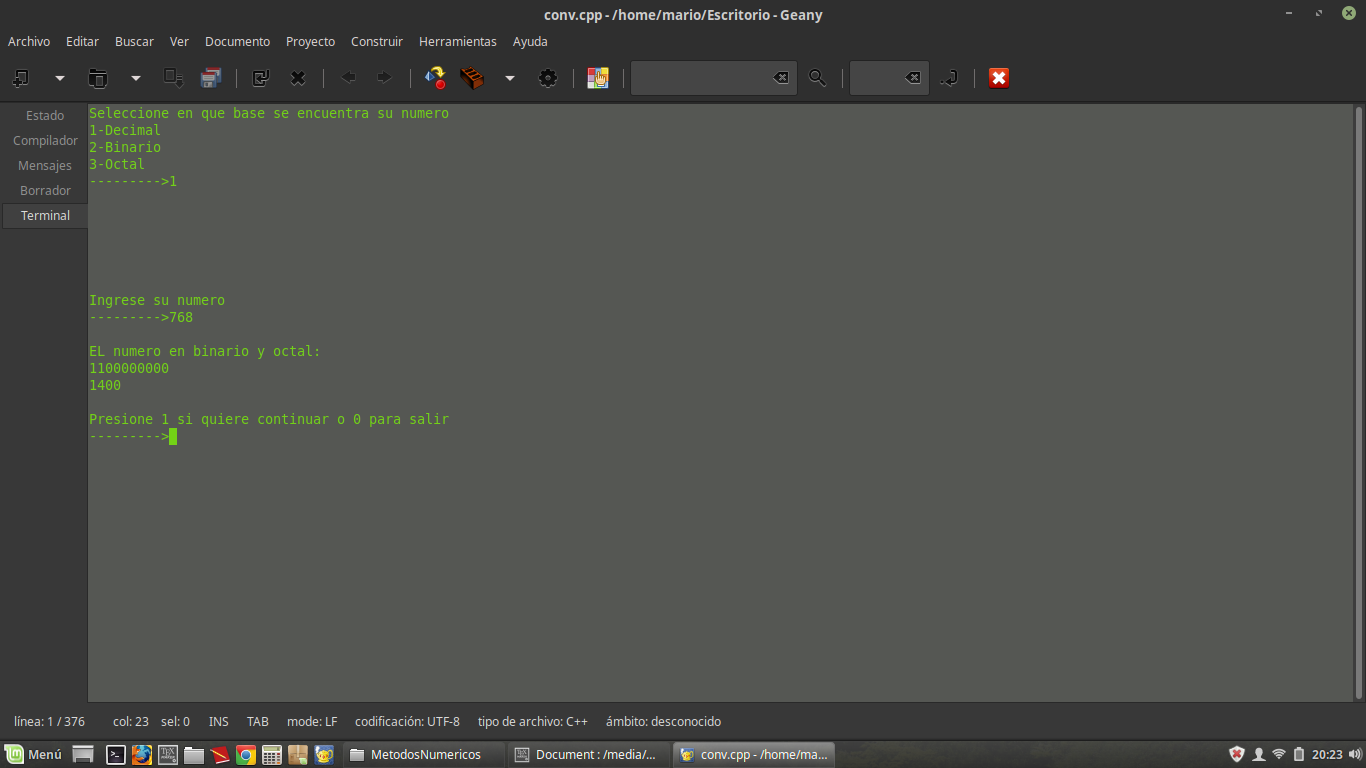
\includegraphics[scale=0.125]{Conversion2.png}
\caption{Parte del programa aplicado}
	\end{figure}
	Como se logra ver en la figura 5 se comprueba que efectivamente la transformacion efectuada es la correcta por lo que se concluye que el programa otorgado es correcto, extendiendose asi para las combianciones entre estos tres tipos de bases.
	
	
\end{multicols}

\end{document}
